\chapter{Architecture}
\label{chap:architecture}


\begin{chapterintro}
This chapter describes in depth how the system is structured in different modules and how the users interact with them and also how the modules interact with other modules by themselves.
\end{chapterintro}

\cleardoublepage
\section{Introduction}
The main purpose of this master thesis is to have a \textbf{repository} of widgets and services to build new mash-ups. First we need to \textbf{feed the repository} and we have to do it automatically using discovery techniques. The content fetched from the internet must be \textbf{structured} before it is inserted into the repository and therefore the repository has to be able to store the data with the same structure, this is done using \textbf{semantic repositories}.

All the information stored in the repository has to be \textbf{managed} manually by an administrator. This is the main goal of this master thesis, create an administration interface that permits an administrator user chose which widgets and services automatically fetched and stored are useful. The administrator interface will provide several tools to the administrator user and will use \textbf{ranking} algorithms to help him decide which ones are usefull.

Finally, there is a web interface for final users that will allow them find services and services using semantic search technologies.

We will fill a semantic repository in a automated way as introduced in section \ref{sec:enableautomated}. To achieve this we use Scrappy~\cite{fernandez2011semantic} explained in section \ref{sec:scrappy}. The former module inserts the semantic data into one of the semantic repositories detailed in section \ref{sec:omrsesame}. This repository needs to be managed by an administrator user through the administrator interface explained in section \ref{sec:omradmin}. The final developer user will access the semantic repository trough the developer or client interface detailed in \ref{subsec:omrclientback}.

A diagram of the architecture is shown in Figure \ref{fig:ArchitectureGeneral}. Each module is detailed in the following sections.

\begin{figure}[ht!]
	\centering
	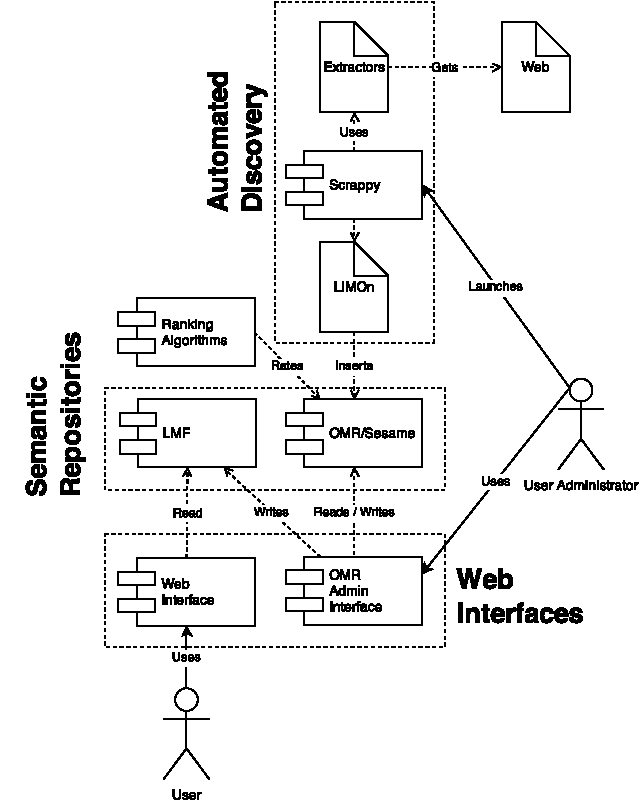
\includegraphics[width=300pt]{graphics/ArchitectureGeneral_v2.pdf}
	\caption{General Architecture}
	\label{fig:ArchitectureGeneral}
\end{figure}

\FloatBarrier

\section{Automated discovery}
\label{sec:scrappy}
The automated discovery module's finality is to fetch several services data from different websites. We fetch this data from \textit{ProgrammableWeb}, \textit{Yahoo! Pipes} and \textit{Opera Widgets}. More information about the type of services and widgets this websites contain is described in section \ref{sec:enableautomated}.

To achieve this we will use Scrappy~\cite{fernandez2011semantic}, an opensource tool  developed by GSI. It can be downloaded from the Github repository of the main contributor of the project\footnote{https://github.com/josei/scrappy}.

It allows us to extract information from web pages and producing RDF data. Within the OMELETTE project, it has been used for developing the Discovery Module and mining several repositories of mashups, widgets and services in order to feed the Omelette Mashup Registry with these components.

Scrappy is developed using Ruby and it uses the Webkit library for visual processing of web resources.

Scrappy access a determined website, gets the corresponding HTML, converts the data into RDF using the defined ontology and inserts the result into the OMR (Figure \ref{fig:scrappysequence}).

\begin{figure}[h]
	\centering
	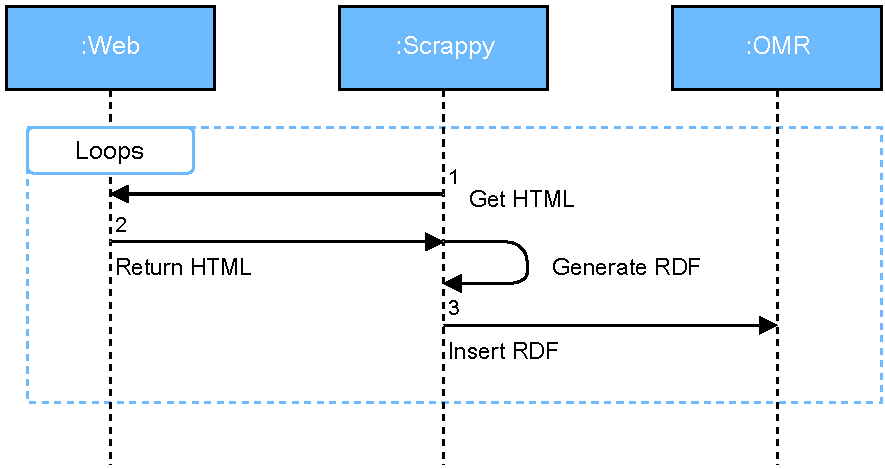
\includegraphics[width=350pt]{graphics/Diagrama_secuencia_scrappy.pdf}
	\caption{Scrappy sequence diagram}
	\label{fig:scrappysequence}
\end{figure}

In order to fetch the desired information from a website, Scrappy needs to know how is the structure of it. This is done by defining a mapping file written in YARF\footnote{format supported by LightRDF gem, as well as RDFXML, JSON, NTriples formats, which can also be used to define the mappings} which reflects the structure of the html file using CSS selectors.

To create the mapping file we need first to analyze manually the HTML. Significant changes in the HTML of the website to be fetched could break the mapping and re-analyzing would be required.

An example of mapping is shown in Listing \ref{lst:extractorExample}, which allows extracting all titles from Yahoo! Pipes.

Scrappy will use the Linked Mashup Ontology (LiMOn) when mapping the resources as seen in \ref{fig:omeletterdfmodel}.

The total number of components scrapped from \textit{Yahoo! Pipes} and \textit{Opera Widgets} can be consulted in table \ref{tab:omrcomsum}.


\begin {table}[ht!]
\caption {Runnable components in OMR} \label{tab:omrcomrun} 
\begin{center}
	\begin{tabular}{|c|c|}
		\hline Number of runnable services                  & 1542          \\ 
		\hline Number of runnable WSDL\footnote{Services containing WSDL descriptions} services             & 296           \\ 
		\hline Number of runnable REST\footnote{Services with REST interface available} services             & 1246          \\ 
		\hline Number of runnable widgets                   & 1804          \\ 
		\hline \textbf{Total number of runnable components} & \textbf{3346} \\ 
		\hline 
	\end{tabular} 
\end{center}
\end{table}

\section{Semantic repository}
\label{sec:omrsesame}
All the services and widgets fetched by the automated discovery module described in the former section \ref{sec:scrappy} have to be stored somewhere. This place is what we call the \textit{OMELETTE Mashup Registry} (OMR).

The objective of the OMELETTE Mashup Registry is to provide an integrated centralized reference of web components to facilitate querying and selection of relevant ones when building new mashups. To achieve this, an RDF model based format is employed to describe the components (see section \ref{subsec:rdfmodel}). 

The registry or repository integrates heterogeneous components that can be potentially used in various web applications. More specifically, mashup applications and services from the Web are the ones under consideration. Mashup is treated as a first-class object that is comprised of any web applications. Examples of mashups and services can be found in repositories such as Yahoo Pipes or Programmable Web.

In order to make these components available for developers, the registry stores relevant metadata that can be used by the developers for selecting components. Additionally, these metadata should be available in the web in order to make it possible to automate the population of the registry with real components. Usually, web component repositories contain metadata such as a component's name, textual description, tags or categorization.

For developing purposes Sesame is used instead of the OMR to help us to solve some problems we were experiencing with different versions of SPARQL. SPARQL is in continuos development and some of the functionalities needed were not implemented in the first 1.0 version but they were in 1.1 version. We chose Sesame between various alternatives as it is one of the most popular.

Both Sesame and OMR complies the same REST API interface.

Sesame is a de-facto standard framework for processing RDF data. This includes parsing, storing, inferencing and querying of/over such data. It offers an easy-to-use API that can be connected to all leading RDF storage solutions.

Sesame has been designed with flexibility in mind. It can be deployed on top of a variety of storage systems (relational databases, in-memory, file systems, keyword indexers, etc.), and offers a large scale of tools to developers to leverage the power of RDF and related standards. Sesame fully supports the SPARQL query language for expressive querying and offers transparent access to remote RDF repositories using the exact same API as for local access. Finally, Sesame supports all main stream RDF file formats, including RDF/XML, Turtle, N-Triples, TriG and TriX.

\section{Ranking module}
\label{sec:rankingmodule}
There are thousands of services and widgets fetched and stored in the semantic repository as shown in Table \ref{tab:omrcomrun}. The administrator user will have to search for useful components in this repository. By default there is no way to distinguish bewteen relevant or not relevant ones. To solve this, we apply the ranking algorithms described by Tilo Zemke~\cite{Tilo12}.

This module is implemented as a separate component written in Java which runs independently. It connects to the semantic repository and executes the algorithms to calculate the indicators in each component. It is scheduled to run periodically and re-calculate the indexes when new mashups or services are incorporated to the meta-directory.

\begin{figure}[h]
	\centering
	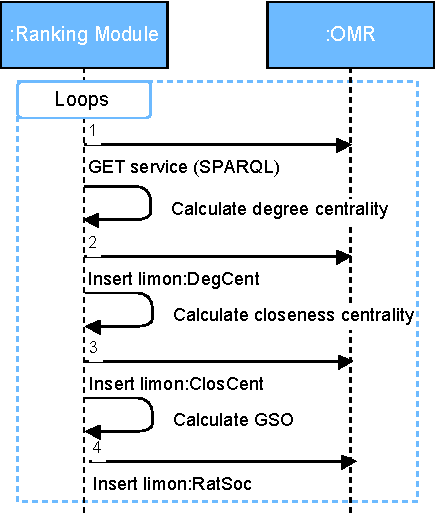
\includegraphics[width=200pt]{graphics/Diagrama_secuencia_ranking.pdf}
	\caption{Sequence diagram for ranking index generation}
	\label{fig:rankingsequence}
\end{figure}

\section{OMR Admin Interface}
\label{sec:omradmin}
The automated discovery module fetches thousands of services and widgets and store them in the semantic repository, therefore they are ranked to make the best matches show up when quering the repository. After this an administrator user has to selelect the appropriate one manually. This must be done within a interface that helps that person to do the job, helping him by browsing trough the different categories and properties defined in the RDF model (section subsec:rdfmodel).

On a first instance we decided to build this interface using Simile Exhibit\footnote{http://simile.mit.edu/wiki/Exhibit}. The description of Exhibit says:

\textit{Exhibit lets you easily create web pages with advanced text search and filtering functionalities, with interactive maps, timelines, and other visualizations}.

That description seemed exactly what we looked for, but some problems occured, for example high load and poor perfomance or unexpected bugs related to non mature technology. We decided to create our own administrator interface based on the principles of Exhibit with faceted search.

\begin{figure}[h]
	\centering
	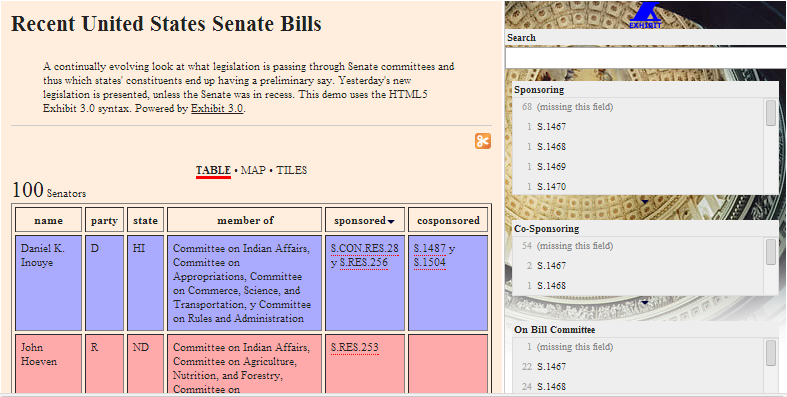
\includegraphics[width=350pt]{graphics/exhibitsimile.png}
	\caption{Simile Exhibit example interface}
	\label{fig:generatingblocks}
\end{figure}

Out OMR administrator interface is  built using PHP\footnote{http://www.php.net}, HTML, CSS and Javascript.

A general view of the class diagram is shown in \ref{fig:admininterface}. All the components are executed from the index.php file, which we will consider as the main file.

One of the big benefits of Exhibit was the easiness for developers to change the main view. The OMR admin interface is done the same way, using the functions library detailed in subsection \ref{subsec:functionslibrary} the developer can change the behavior and functionalities of the web interface.

\begin{figure}[ht!]
	\centering
	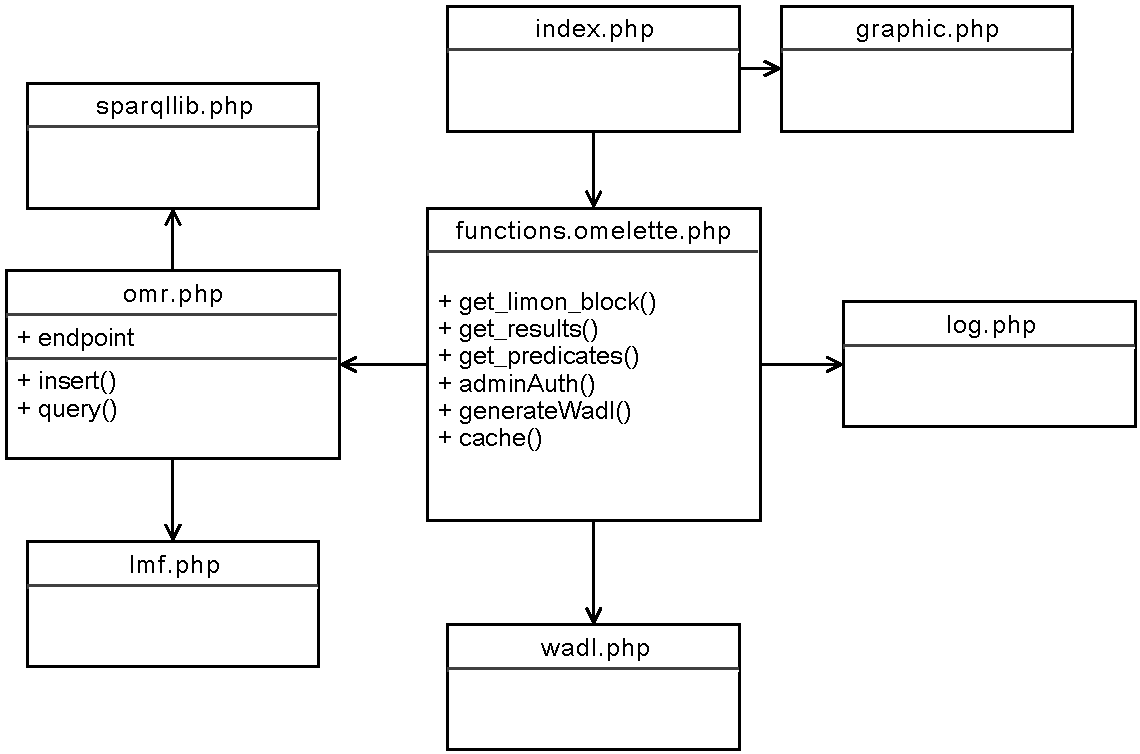
\includegraphics[width=400pt]{graphics/omr-interface-architecure.pdf}
	\caption{OMR Admin Interface architecture}
	\label{fig:admininterface}
\end{figure}

\FloatBarrier

\subsection{Main component}
The main file of the OMR Admin interface is the \textit{index.php}. It is the execution point. The rest of components and functions are called from this execution point.

In the \textit{index.php} the developer can decide how to visualize everything and just adding few lines of code it will generate the facet boxes and the results container.

It is mostly HTML with CSS and Javascript. It also uses the javascript framework jQuery\footnote{http://jquery.com} and svglizer\footnote{http://sgvizler.googlecode.com/} to render the result of SPARQL SELECT queries into charts.

The functions available that will generate the HTML automatically are described in \textit{functions.omelette.php} and will be detailed in the sub-section \ref{subsec:functionslibrary}.

\begin{figure}[ht!]
	\centering
	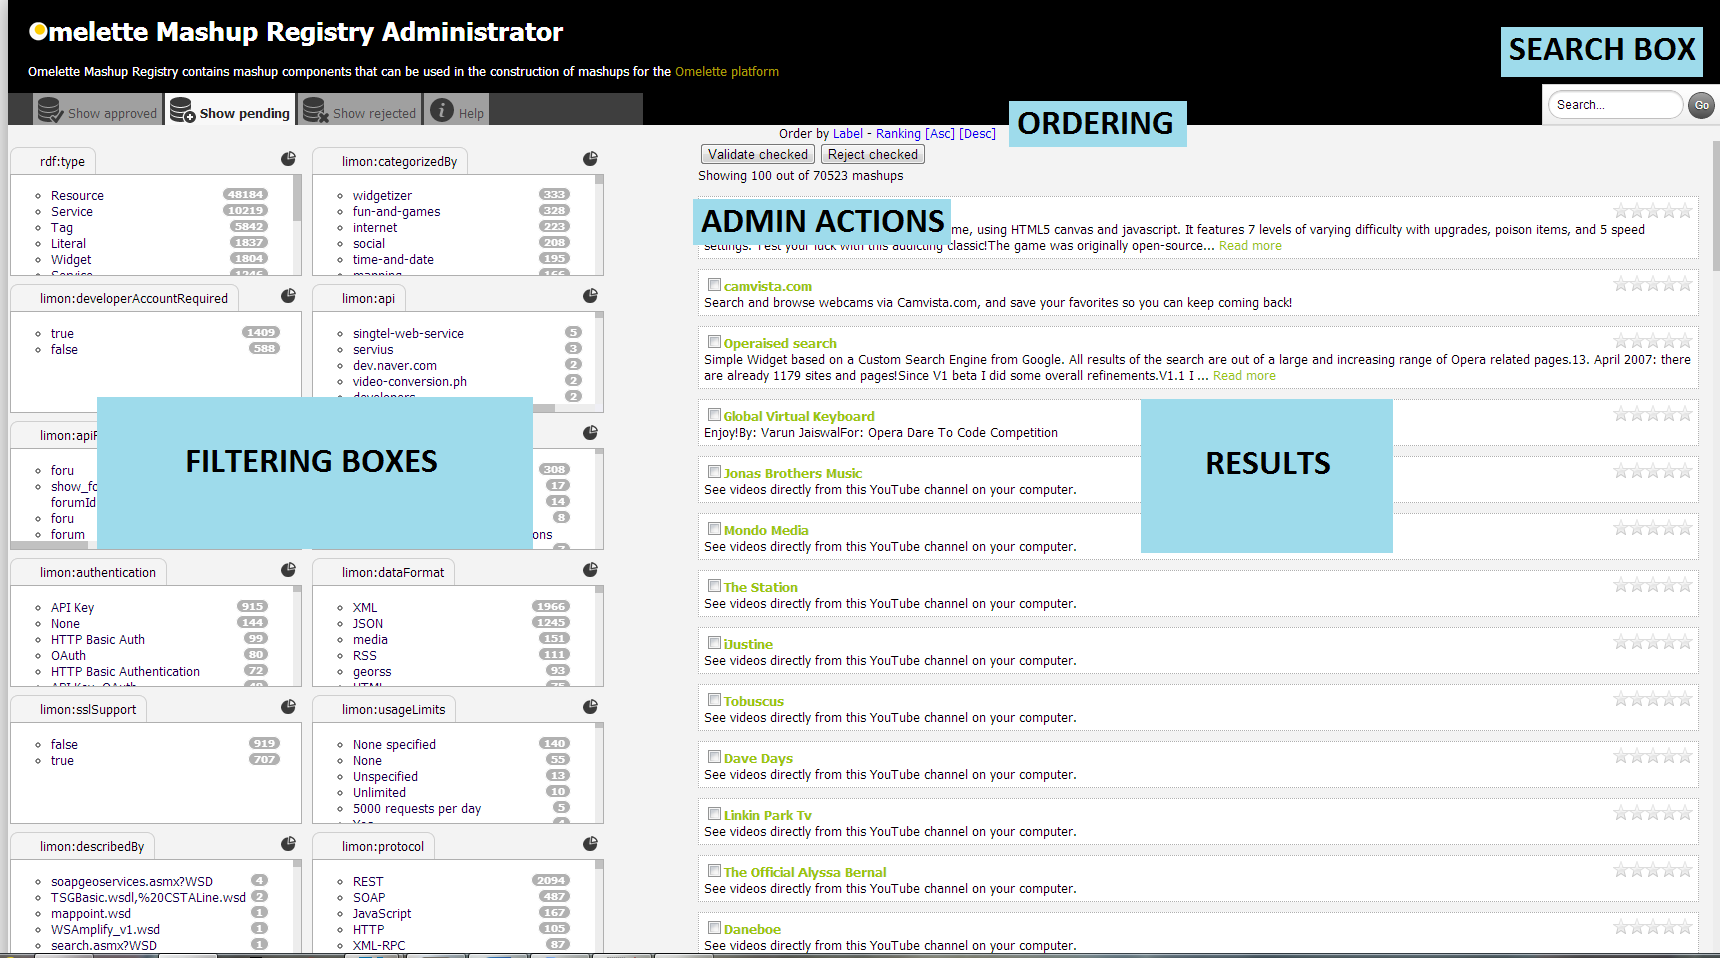
\includegraphics[width=400pt]{graphics/omr-admin.png}
	\caption{OMR Admin Interface}
	\label{fig:admininterfacemain}
\end{figure}
\subsection{Functions library}
\label{subsec:functionslibrary}
The file \textit{functions.omelette.php} is a library of functions used by the rest of the classes. These functions will help to generate the HTML code in the interface.

\subsubsection{Facet boxes}
This is one of the functions of the library. By creating facet boxes we can do facet searching. We can create one facet box for each of the properties defined in the RDF model (section \ref{subsec:rdfmodel}).

We can create facet boxes using the following function in the main file of our interface. Every time we call the \textit{get\_limon\_block()} function it will render a facet box.

\begin{lstlisting}[breaklines=true, style=mono, caption="Creating facet box"]
<?php get_limon_block("limon:categorizedBy",filter); ?>
\end{lstlisting}

In the Figure \ref{fig:generatingblocks} we can see the code on the right that will render the facet boxes on the left.

\begin{figure}[h]
	\centering
	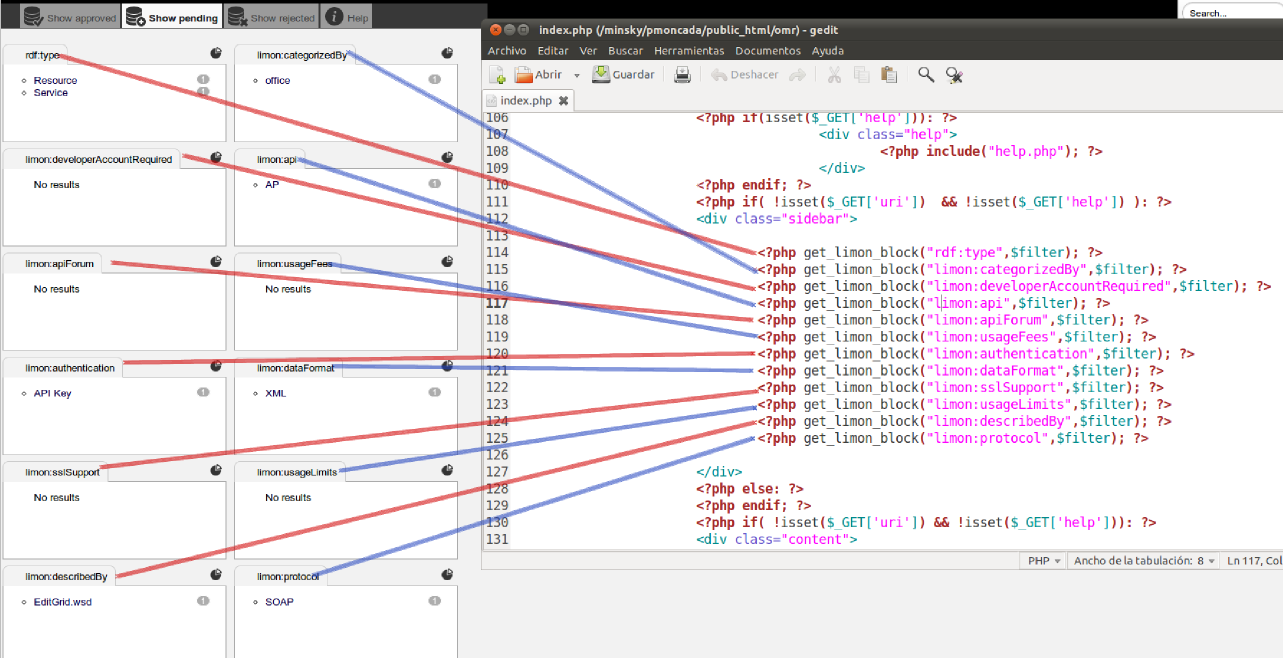
\includegraphics[width=400pt]{graphics/generatingblocks.png}
	\caption{Generating Facet Boxes}
	\label{fig:generatingblocks}
\end{figure}

\newpage
\subsubsection{Result lists}
The results of the search are shown in the \textit{result list}. We can create a result list container with the following PHP function of the library:

\begin{lstlisting}[breaklines=true, style=mono, caption="Creating result container"]
<?php get_results(filter,order,dir); ?>
\end{lstlisting}

\subsubsection{Widget or service}
If we want to see all the information regarding to a selected \textit{widget or service} we can do it by using the code listed here. This information is showed when clicking on a hyperlink of the result list.

\begin{lstlisting}[breaklines=true, style=mono, caption="Creating information view"]
				<?php elseif( isset(_GET['uri']) ): ?>
					<?php get_predicates(_GET['uri']); ?>				
				<?php endif; ?>
\end{lstlisting}

\subsubsection{Generate charts}
We can generate charts to see in a graphical way the information regarding to the repository as different services shown in different categories.

It uses an external module named \textit{svglizer} to generate charts. The system will generate the proper SPARQL SELECT query and insert it into the module to generate the pie chart.

\begin{lstlisting}[breaklines=true, style=mono, caption="Generating pie charts"]
<div id="chart"
      data-sgvizler-endpoint="http://krusti.gsi.dit.upm.es:8080/LMF-3.0.0/sparql/select"
      data-sgvizler-query="<?php echo base64_decode(_GET['query']); ?>"
      data-sgvizler-chart="gPieChart"
      data-sgvizler-endpoint_output="xml" 
      style="width:800px; height:400px;"></div
	</body>
\end{lstlisting}

\begin{figure}[h]
	\centering
	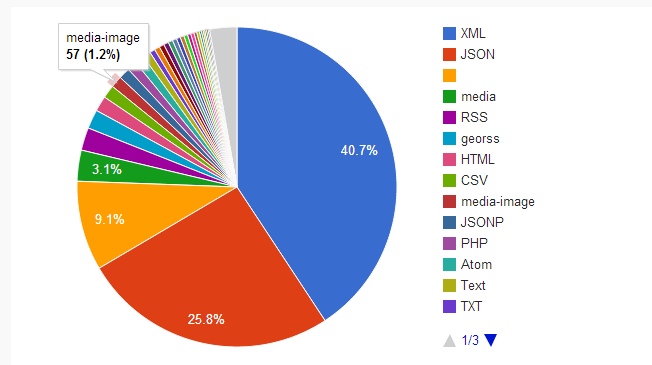
\includegraphics[width=300pt]{graphics/piechart.png}
	\caption{Pie chart}
	\label{fig:piechart}
\end{figure}

To generate a chart to visualize statistics, the user has to browse trough the OMR administrator, selecting filters and making search queries using free text. When the user is satisfied with the results showed he can cick on the button to generate the pertinent chart. The flow can be visualized in figure \ref{fig:chartsequence}.

\begin{figure}[h]
	\centering
	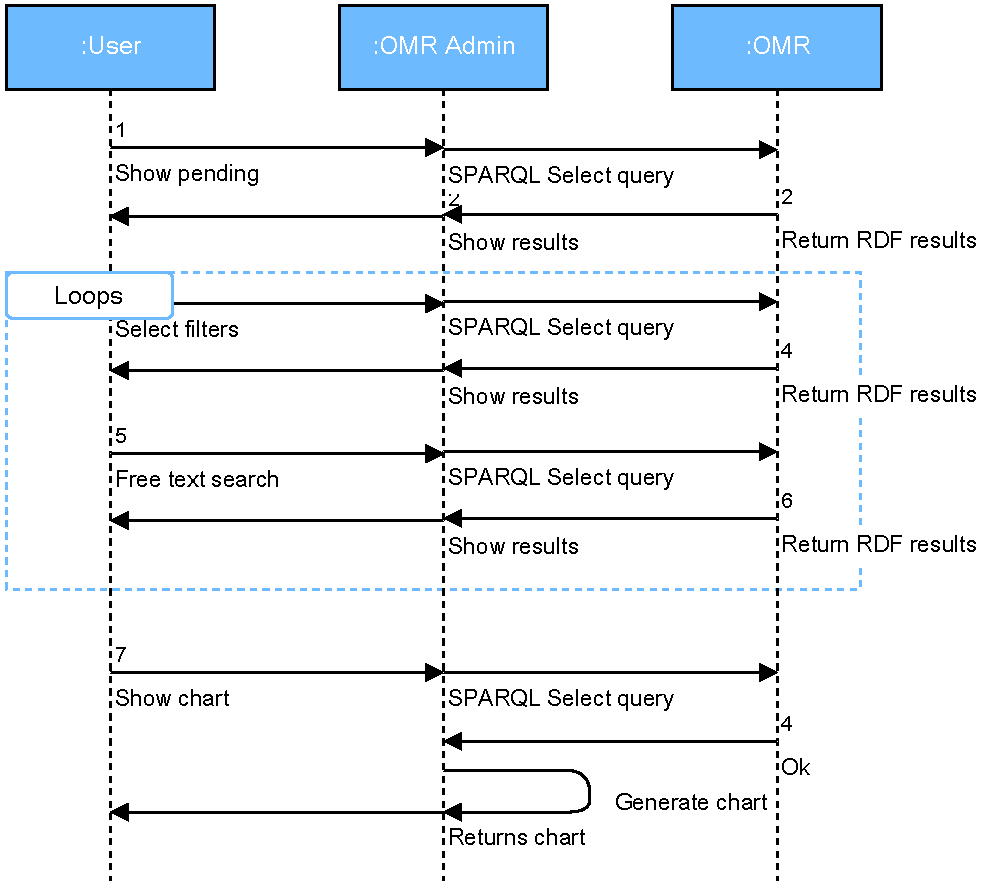
\includegraphics[width=350pt]{graphics/Diagrama_secuencia_graficas.pdf}
	\caption{Sequence diagram for chart generation}
	\label{fig:chartsequence}
\end{figure}

\subsubsection{Admin authentication}
The OMR Admin interface provides of basic athentication for write operations on the repository. This authentication is HTTP based\footnote{http://php.net/manual/es/features.http-auth.php} using PHP.


\subsubsection{Cache and performance}
\label{subsubsec:cacheperfomance}
When working with thousands of components in the semantic repository some perfomance issues came up. To solve this we created some helpers written as funtions inside the library that creates a file based cache.

The cache system works as follows. When a query to the OMR is executed (Figure \ref{fig:cachesequence_a}) it stores the result shown in \ref{lst:cachecat} using a no collision hash calculated using the SPARQL query. Every time a query is launched it will look for a stored result in the cache file list \ref{lst:cachels} and it will be served in case there is a matching (Figure \ref{fig:cachesequence_b}). The cached result is parsed the same way using sparqllib.
This is quite important when working with a repository with thousands of services that will demand high processing time for all of them to be retrieved and filtered.

\begin {table}[ht!]
\caption {Execution query time comparison} \label{tab:timecomp} 
\begin{center}
	\begin{tabular}{|c|c|c|c|}
		\hline              & OMR Quering & Local Sesame & Cached query \\ 
		\hline Maximun time & 120 seconds & 15 seconds   & ~0 seconds   \\ 
		\hline Minimun time & 3 secods    & 1 second     & ~0 seconds   \\ 
		\hline 
	\end{tabular}
\end{center}
\end{table}


\begin{figure}[h]
	\centering
	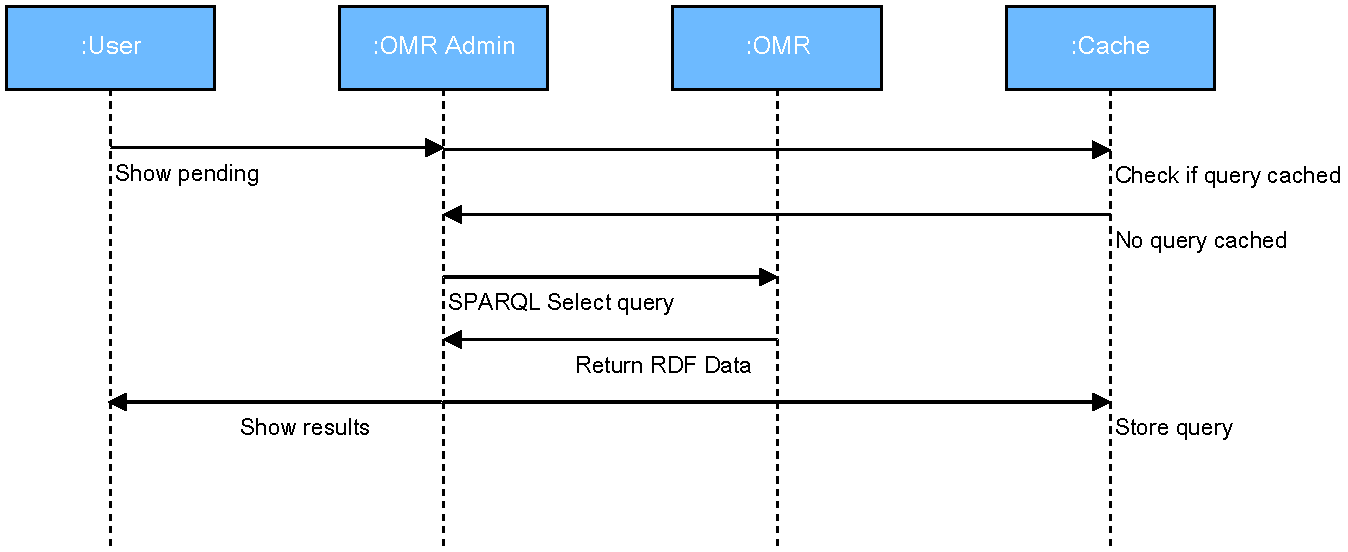
\includegraphics[width=350pt]{graphics/Diagrama_secuencia_cache_A.pdf}
	\caption{Sequence diagram if query is not in cache}
	\label{fig:cachesequence_a}
\end{figure}

\begin{figure}[h]
	\centering
	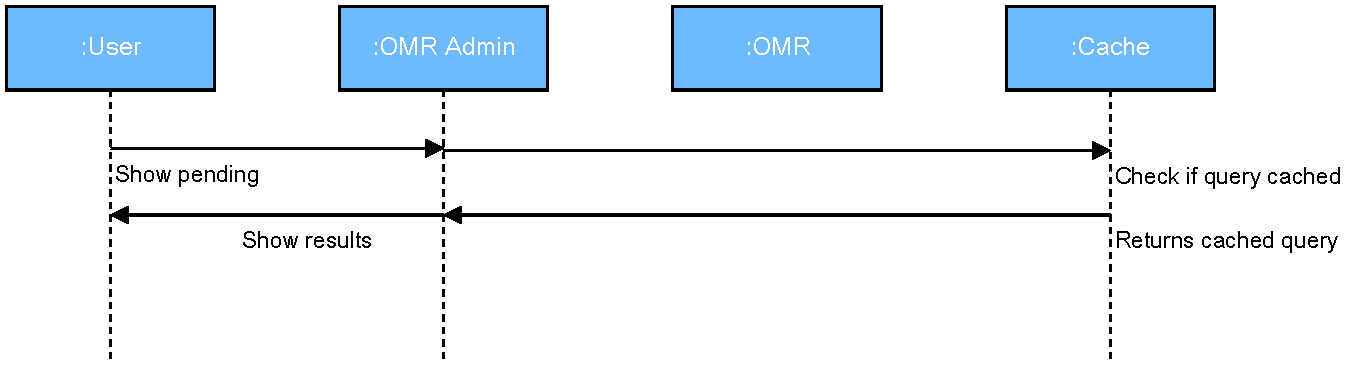
\includegraphics[width=350pt]{graphics/Diagrama_secuencia_cache_B.pdf}
	\caption{Sequence diagram if query cached}
	\label{fig:cachesequence_b}
\end{figure}
\FloatBarrier
\lstinputlisting[caption={Cache file list example},label={lst:cachels},style={consola} ]{code/cache_ls.txt}
\lstinputlisting[caption={Cache file out example},label={lst:cachecat},style={consola} ]{code/cache_cat.txt}

\subsubsection{Repository wrapper}
To connect to the semantic repository we use a wrapper that is in charge to do it using the \textit{sparql library} (sub-section \ref{subsubsec:sparqllibrary}) and also using the cache system described in sub-section \ref{subsubsec:cacheperfomance}.

The class omr.php allows allows the system to connect to the different repositories available providing an API to it.
\begin{itemize}
	\item connect(), connects to the repository endpoint.
	\item query(), executes a query in SPARQL language
	\item insert(), inserts a new element into the repository.
\end{itemize}

The posible repositories are the OMR, Sesame and LMF.\footnote{Linked Media Framework}


\subsubsection{Sparql Library}
\label{subsubsec:sparqllibrary}
In order to handle RDF processing and SPARQL queries responses parsing, the system uses a third party library, sparqllib.php\footnote{http://graphite.ecs.soton.ac.uk/sparqllib/}.

It has been modified to allow queries using POST method and HTTP authentication (which is a requisite for connecting to the OMR).

The library provides functions very similar to PHP mysql\_* for comfort.

\lstinputlisting[label=sparqllibsample,caption=Sparqllib usage example,style={consola} ]{code/sparqllib_example.php}

\begin {table}[ht!]
\caption {Sparqllib output example} \label{tab:sparqllibsample} 
\begin{center}
	\begin{tabular}{|c|c|}
		\hline 
		Person          & Name  \\ 
		\hline 
		bf4120a00000000 & Bob   \\ 
		\hline 
		bf4120a1200000e & Alice \\ 
		\hline 
	\end{tabular}
\end{center}
\end{table}
The output is shown in Table \ref{tab:sparqllibsample}

\newpage

\subsubsection{Validating resource}
\label{subsubsection:validationresourcearch}
The users browses into the repository trough the OMR admin interface going into the "Browse pending" section (Figure \ref{fig:admintopmenu}), selecting filters from the facet boxes (Figure \ref{fig:generatingblocks}) and using the free text search box (Figure \ref{fig:searchboxadmin}) finally reaches a resource to be validated. 

\begin{figure}[h]
	\centering
	
\includegraphics[width=200pt]{graphics/admin-top-menu.png}
	\caption{OMR admin top menu}
	\label{fig:admintopmenu}
\end{figure}

When selecting the validate button (Figure \ref{fig:validatebutton}), a SPARQL update query will be executed using the Sparql library to modify the OMR to indicate that the selected resource is already validated. Additionally, the RDF resource will be stored into the LMF to be indexed by SOLR.

\begin{figure}[h]
	\centering
	
\includegraphics[width=200pt]{graphics/omr-validate-buttons.png}
	\caption{OMR admin validate and reject buttons}
	\label{fig:validatebutton}
\end{figure}

Then, the validated services are shown in the \textit{Show approved} section that can be accessed through the top menu as seen in Figure \ref{fig:admintopmenu}.

The whole sequence is shown in Figure \ref{fig:validatesequence}.
%\begin{figure}[h]
%\centering
%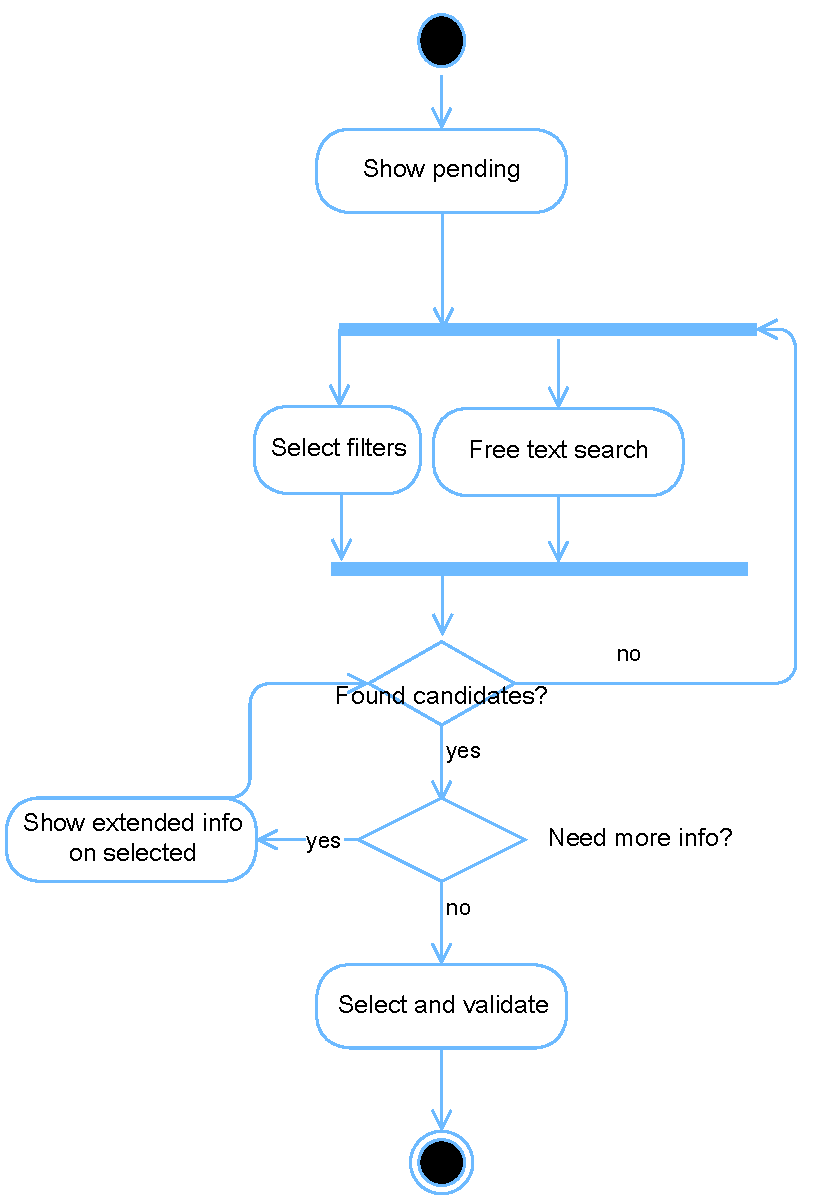
\includegraphics[width=350pt]{graphics/validar_servicio.pdf}
%\caption{Activity diagram for validating service}
%\label{fig:validateactivity}
%\end{figure}


\begin{figure}[h]
	\centering
	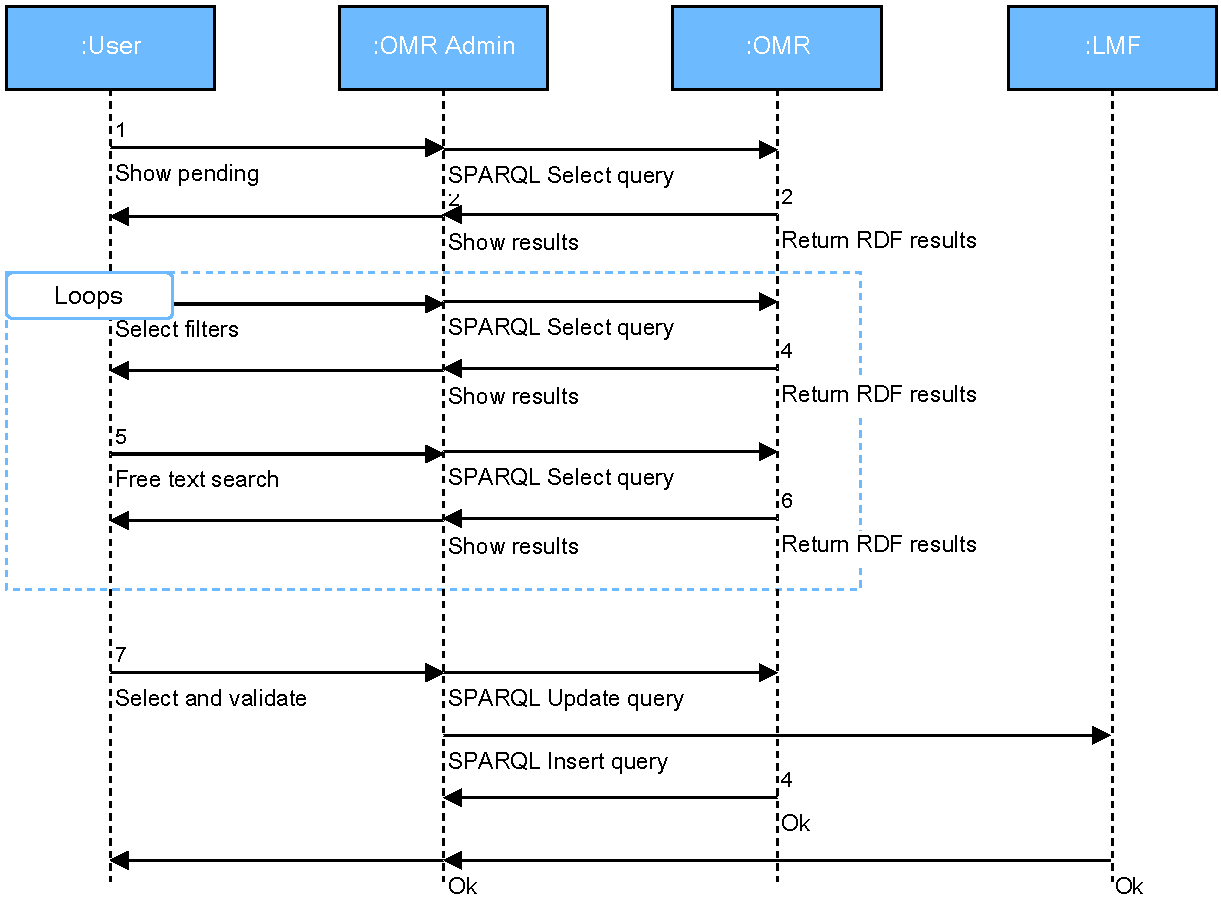
\includegraphics[width=350pt]{graphics/Diagrama_secuencia_validar.pdf}
	\caption{Sequence diagram for validating RDF resource}
	\label{fig:validatesequence}
\end{figure}
\newpage
\subsubsection{Rejecting resource}
The users browses into the repository trough the OMR admin interface going into the "Browse pending" section (Figure \ref{fig:admintopmenu}), selecting filters from the facet boxes (Figure \ref{fig:generatingblocks}) and using the free text search box (Figure \ref{fig:searchboxadmin}) finally reaches a resource to be validated. When selecting the reject button (Figure \ref{fig:validatebutton}), a SPARQL update query will be executed using the Sparql library to modify the OMR to indicate that the selected resource has been rejected by the administrator.

\begin{figure}[h]
	\centering
	
\includegraphics[width=100pt]{graphics/omr-search-box.png}
	\caption{OMR admin search box}
	\label{fig:searchboxadmin}
\end{figure}

\begin{figure}[h]
	\centering
	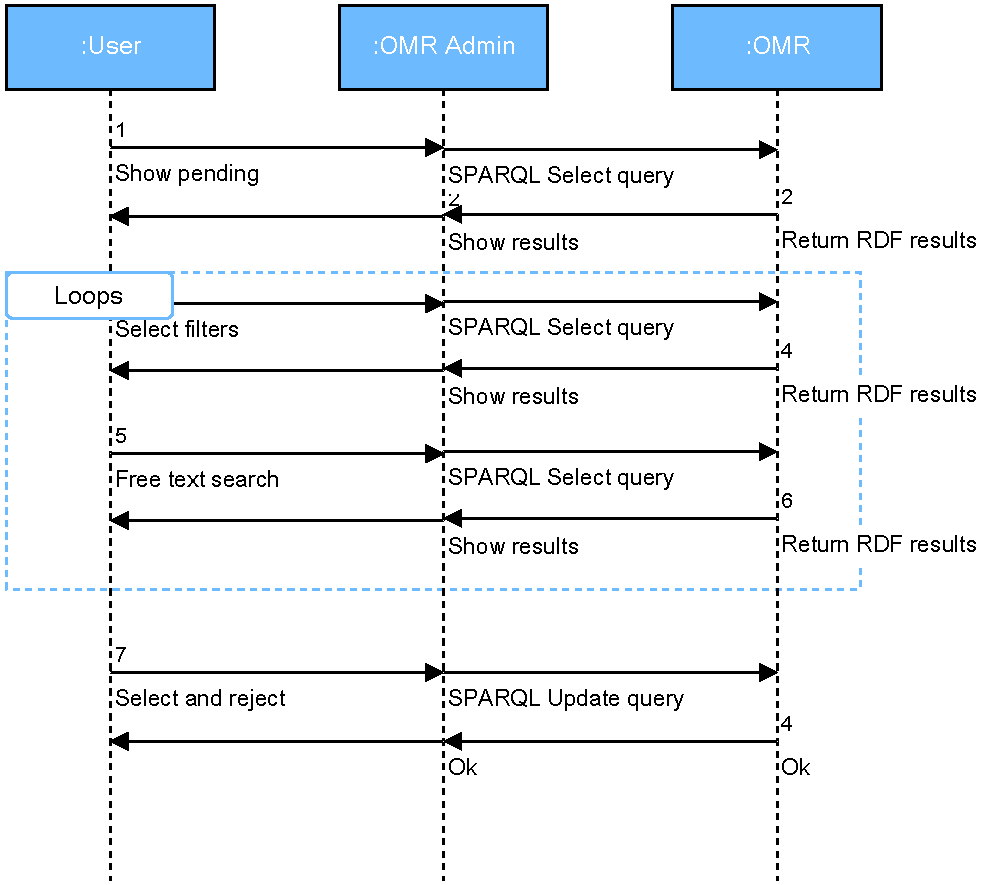
\includegraphics[width=350pt]{graphics/Diagrama_secuencia_rechazar.pdf}
	\caption{Sequence diagram for rejecting RDF resource}
	\label{fig:rejectsequence}
\end{figure}

\newpage
\subsubsection{Wadl generation}
The system can generate a WADL\footnote{ is a machine-readable XML description of HTTP-based web applications (typically REST web services)} file for those services with rosm\footnote{http://www.wsmo.org/ns/rosm/0.1/} description.
\textbf{Important}: This is only available for services scrapped from Yahoo Pipes.

It returns a WADL file where it is specified the target URL and parameters for the REST service.
This data is easily fetched executing SPARQL query as shown in \ref{lst:wadlsparql}.
\newpage
\begin{lstlisting}[breaklines=true, style=consola, caption={Retrieving information for WADL with SPARQL}, label={lst:wadlsparql}]
SELECT DISTINCT ?parameter ?getUrl WHERE{
	 uriresource limon:describedBy ?a .
	 ?a rosm:supportsOperation ?b .
	 ?b hrests:hasAddress ?getUrl .
	 ?b rosm:requestURIParameter ?c .
	 ?c rdfs:label ?d .
	 ?d rdfs:label ?parameter	 
	}
\end{lstlisting}

An example of WADL output is shown in \ref{lst:wadlexample}.


\lstinputlisting[label=example-wadl,caption=WADL example,label={lst:wadlexample},style={consola} ]{code/example-wadl.xml}

To generate WADL, the user has to browse trough the OMR Admin and select a mashup or service. Afterwards, if it is supported by the selected service, the user can request the OMR Admin to generate a WADL file. This sequence is described in figure \ref{fig:wadlsequence}.

\begin{figure}[h]
	\centering
	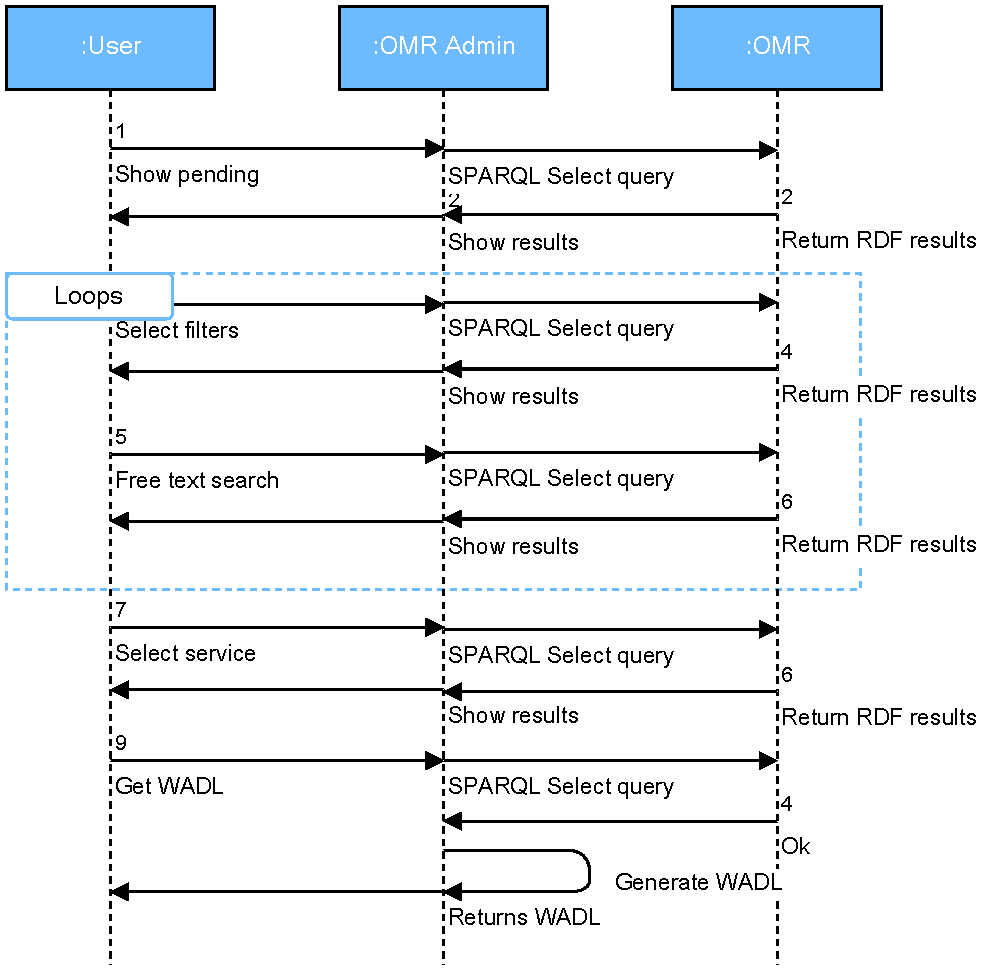
\includegraphics[width=350pt]{graphics/Diagrama_secuencia_wadl.pdf}
	\caption{Sequence diagram for WADL file generation}
	\label{fig:wadlsequence}
\end{figure}

\FloatBarrier

\subsubsection{LMF integration}
There is an extra module\footnote{lmf.php} that adapts the queries to insert selected services into an LFM repository. This enables SOLR indexing for the client service browser.

It connects to the sparql/update endpoint of LMF, in wich SPARQL insert queries can be executed.


\section{OMR Client Browser}
\label{sec:omrclientbrowser}

This interface is used by the final user when he wants to find suitable widgets or services to build new mash-ups. It connects to the repository and reads the components approved formerly by the administrator user via the OMR Admin interface.

The OMR Client Browser (\ref{fig:omrclient}) consists in two parts, a back-end formed by LMF, and a front-end written using web technologies such as javascript and HTML.
It is based on the Episteme\footnote{Episteme is a creator of opportunities designed to link the various partners and create consortia to suit a particular offer. With semantic search is able to find companies that are the best suited to an opportunity based on their characteristics.} platform.

The user can create a new search which will be automatically saved for posterity. The user will be shown a form with auto complete fields (which will retrieve the auto-complete data automatically (step 2 in Figure \ref{fig:clientsequence}). The user selects the desired filters (step 3 in Figure \ref{fig:clientsequence}). A HTTP request to the LMF is made to retrieve the search results (step 4 in Figure \ref{fig:clientsequence}). If any of the fields was semantic, an extra HTTP request will be done to the semantic module. The results are shown to the user (step 5 in Figure \ref{fig:clientsequence}).
\begin{figure}[h]
	\centering
	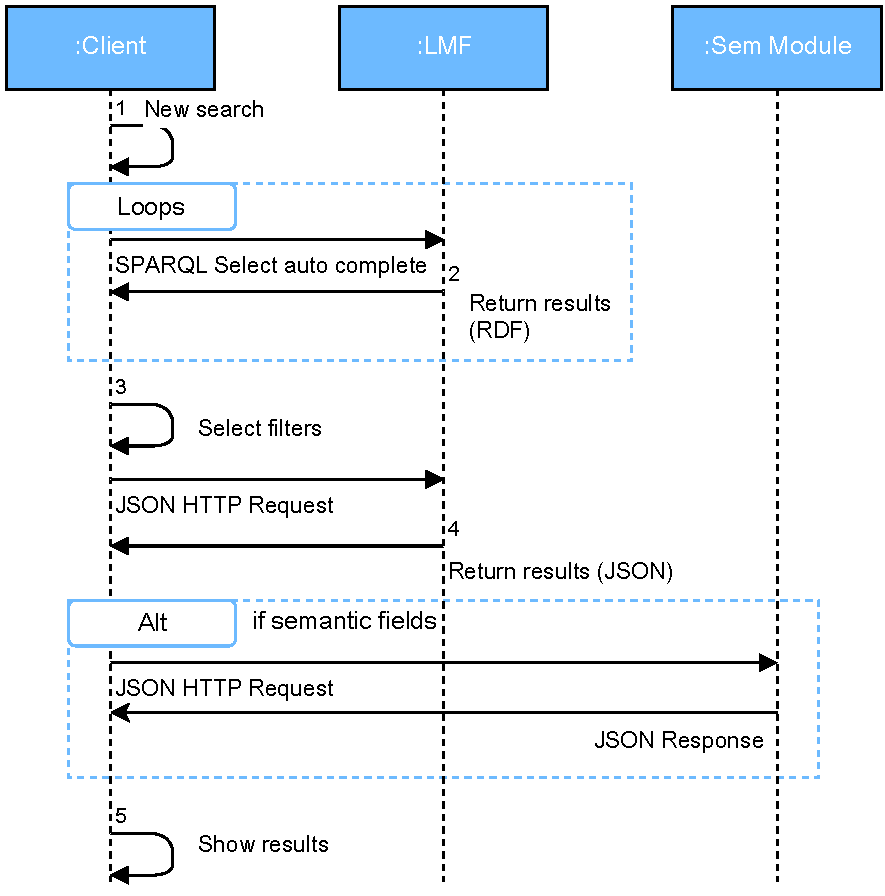
\includegraphics[width=350pt]{graphics/Diagrama_secuencia_client.pdf}
	\caption{Scrappy sequence diagram}
	\label{fig:clientsequence}
\end{figure}

All the modules are described in the following points.

%TODO hacer mas alta esta imagen y menos ancha
\begin{figure}[ht!]
	\centering
	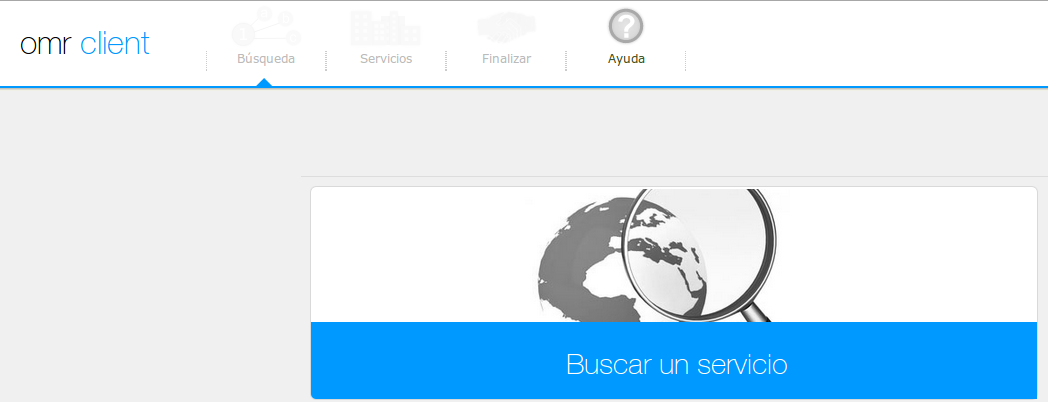
\includegraphics[width=460px]{graphics/omrclient.png}
	\caption{OMR client interface}
	\label{fig:omrclient}
\end{figure}



\subsection{Back-end}
\label{subsec:omrclientback}
For the back-end the system uses Linked Media Framework to build semantic search over the approved data selected with the OMR Admin described in \ref{sec:omradmin}.
The only thing needed to configure the LMF is a semantic core that should follow the rules showed in \ref{lst:semcore}. A search core represents a specific index configuration with fields filled from the linked data cloud. It consists of two mayor elements: a filter deciding which resources are added to the search index, and one or more fields defining the index fields of the search core and how the values of these fields are calculated.
These filters are written following LD Path\footnote{http://code.google.com/p/ldpath/}, a simple path-based query language, similar to SPARQL Property Paths, that is particularly well-suited for querying and retrieving resources from the Linked Data Cloud by following RDF links between resources and servers.

\newpage

\begin{lstlisting}[breaklines=true, style=consola, caption={Semantic core configuration for LMF using LD Path}, label={lst:semcore}]
@prefix limon : <http://www.ict-omelette.eu/schema.rdf#> ;
@prefix ctag : <http://commontag.org/ns#>;
  
  Rdftype = rdf:type :: xsd:string ;
  categorizedBy = limon:categorizedBy :: xsd:string ;
  api = limon:api :: xsd:string ;
  sslSupport = limon:sslSupport :: xsd:string ;
  label = rdfs:label :: xsd:string ;
  protocol = limon:protocol :: xsd:string ;
  tagged = ctag:tagged :: xsd:string ;
  authentication = limon:authentication :: xsd:string ;
  dataFormat = limon:dataFormat :: xsd:string ;
  description = dc:description :: xsd:string ;
  Provenance = "gsi" :: xsd:string ;
\end{lstlisting}

\subsection{Front-end}
\label{subsec:omrclientfront}
The Episteme front-end has been developed using various JavaScript frameworks, such as Knockout JS which simplifies the dynamic JavaScript UI with the Model-View-View Model (MVVM) pattern, and KendoUI\footnote{http://www.kendoui.com} to build beautiful interactive interface.
Creating a search engine with Episteme has been done following few steps.

\paragraph{Search fields} If we want to show new search fields as shown in figure \ref{fig:searchfields} first of all we have to construct the SPARQL query that will fill the auto-complete. For example, one of them should look like described in \ref{lst:sparqlauto}. It is also necessary to add the data binding sequence with knockout as shown in \ref{lst:databinding}.

\newpage

\begin{lstlisting}[breaklines=true, style=consola, caption={SPARQL to retrieve all component types}, label={lst:sparqlauto}]
SELECT DISTINCT ?o  
  WHERE { ?a rdf:type ?o . } 
  GROUP BY ?o ORDER BY DESC(?o) 
}
\end{lstlisting}

\begin{figure}[h]
	\centering
	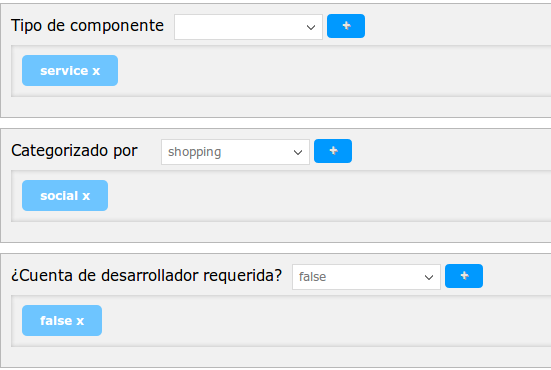
\includegraphics[width=300px]{graphics/searchfields.png}
	\caption{Search fields in OMR client interface}
	\label{fig:searchfields}
\end{figure}
\begin{lstlisting}[breaklines=true, style=listXML, caption={Data binding with knockout}, label={lst:databinding}]
<!-- RDF TYPE -->
    <span data-bind="if: data.field() == 'Rdftype'">
      <span class="filterName" data-bind="text: root.lang().rdftype"></span>
      <input class="solrInput" data-bind="kendoComboBox: { data: root.Rdftype, value: root.selectedRdftype}" />
      <a class="greenButton" data-bind="click: root.addSolrFilter.bind(data, data.values, root.selectedRdftype)">+</a>
      <a class="filterInfo blueButton" data-bind="click: root.addSolrFilter.bind(data, data.values, root.selectedType),attr: { 'title': root.lang().rdftypeHelp}">?</a>
    </span>
\end{lstlisting}
\paragraph{Multilingual support}Episteme is prepared to enable multi-language, all the string values are stored in the \textit{dictionary.js}.
\paragraph{Personalization manual} is available with full detail at the Episteme Wiki.\footnote{https://github.com/gsi-upm/Episteme/wiki/Create-a-custom-search-engine-with-Episteme}


\section{Conclusions}
We have shown a architecture fully modular in which each component can be developed, maintained and deployed separately.

The automated discovery system could be upgraded to acquire  new functionalities and adapt to new web structure.

As we demonstrated the OMR module could be substituted by an other framework to store the RDF data such as Sesame as we built the communication interface complying the standards.

Using modules built using the Model-View-View Model patters makes them reusable and extended for other purposes.

All modules are available as open source projects.

\begin{itemize}
\item Sesame: http://www.openrdf.org/download.jsp
\item LMF: https://code.google.com/p/lmf/downloads
\item Scrappy: https://github.com/gsi-upm/scrappy
\item OMR admin: https://github.com/gsi-upm/omr-admin
\item OMR client: https://github.com/gsi-upm/omr-client
\end{itemize}
